%%%%%%%%%%%%%%%%%%%%%%%%%%%%%%%%%%%%%%%%%%%%%%%%%%%%%%%%%%%%%%%%%%%%%%%%%%%%%%%%
%%%%%%%%%%%%%%%%%%   Vorlage für eine Abschlussarbeit   %%%%%%%%%%%%%%%%%%%%%%%%
%%%%%%%%%%%%%%%%%%%%%%%%%%%%%%%%%%%%%%%%%%%%%%%%%%%%%%%%%%%%%%%%%%%%%%%%%%%%%%%%

% Erstellt von Maximilian Nöthe, <maximilian.noethe@tu-dortmund.de>
% ausgelegt für lualatex und Biblatex mit biber

% Kompilieren mit
% latexmk --lualatex --output-directory=build thesis.tex
% oder einfach mit:
% make

\documentclass[
  tucolor,       % remove for less green,
  BCOR=6mm,     % 12mm binding corrections, adjust to fit your binding
  parskip=half,  % new paragraphs start with half line vertical space
  open=any,      % chapters start on both odd and even pages
  cleardoublepage=plain,  % no header/footer on blank pages
  bibliography=totoc,
]{tudothesis}
% Seitenraender anpassen
 \usepackage{geometry}
 \geometry{
 left=3cm,
 right=3cm,
 top=3cm,
 bottom=3.7cm,
 bindingoffset=6mm
}


% Warning, if another latex run is needed
\usepackage[aux]{rerunfilecheck}
\usepackage{listings}
% just list chapters and sections in the toc, not subsections or smaller
%\setcounter{tocdepth}{1}

%------------------------------------------------------------------------------
%------------------------------ Fonts, Unicode, Language ----------------------
%------------------------------------------------------------------------------
\usepackage{fontspec}
\defaultfontfeatures{Ligatures=TeX}  % -- becomes en-dash etc.

% load english (for abstract) and ngerman language
% the main language has to come last
\usepackage[american, ngerman]{babel}

% intelligent quotation marks, language and nesting sensitive
\usepackage[autostyle]{csquotes}

% microtypographical features, makes the text look nicer on the small scale
\usepackage{microtype}

%------------------------------------------------------------------------------
%------------------------ Math Packages and settings --------------------------
%------------------------------------------------------------------------------

\usepackage{amsmath}
\usepackage{amssymb}
\usepackage{mathtools}

\usepackage[
version=4,
math-greek=default,
text-greek=default,
]{mhchem}

% Enable Unicode-Math and follow the ISO-Standards for typesetting math
\usepackage[
  math-style=ISO,
  bold-style=ISO,
  sans-style=italic,
  nabla=upright,
  partial=upright,
  warnings-off={mathtools-colon,mathtools-overbracket}, % suppress some unnecessary warnings
]{unicode-math}
\setmathfont{Latin Modern Math}

% nice, small fracs for the text with \sfrac{}{}
\usepackage{xfrac}


%------------------------------------------------------------------------------
%---------------------------- Numbers and Units -------------------------------
%------------------------------------------------------------------------------

\usepackage[
  locale=DE,
  separate-uncertainty=true,
  per-mode=symbol-or-fraction,
]{siunitx}

%------------------------------------------------------------------------------
%-------------------------------- tables  -------------------------------------
%------------------------------------------------------------------------------

\usepackage{booktabs}       % \toprule, \midrule, \bottomrule, etc

%------------------------------------------------------------------------------
%-------------------------------- graphics -------------------------------------
%------------------------------------------------------------------------------

\usepackage{graphicx}
% currently broken
% \usepackage{grffile}

% allow figures to be placed in the running text by default:
\usepackage{scrhack}
\usepackage{float}
\floatplacement{figure}{htbp}
\floatplacement{table}{htbp}

% keep figures and tables in the section
%\usepackage[section, below]{placeins}

% allows to include PDFs as full pages
\usepackage{pdfpages}

% Set the PDF Version of this document to 1.7 (1.4 is the current default)
% This is needed so that PDFs with Version >1.5 can be included
\pdfvariable minorversion=7

%------------------------------------------------------------------------------
%---------------------- customize list environments ---------------------------
%------------------------------------------------------------------------------

\usepackage{enumitem}

%------------------------------------------------------------------------------
%------------------------------ Bibliographie ---------------------------------
%------------------------------------------------------------------------------

\usepackage[
  backend=biber,   % use modern biber backend
  autolang=hyphen, % load hyphenation rules for if language of bibentry is not
                   % german, has to be loaded with \setotherlanguages
                   % in the references.bib use langid={en} for english sources
]{biblatex}
\addbibresource{../references.bib}  % the bib file to use
\addbibresource{../programme.bib}
\DefineBibliographyStrings{german}{andothers = {{et\,al\adddot}}}  % replace u.a. with et al.


% Last packages, do not change order or insert new packages after these ones
\usepackage[pdfusetitle, unicode, linkbordercolor=tugreen, citebordercolor=tugreen]{hyperref}
\usepackage{bookmark}
\usepackage[shortcuts]{extdash}

%------------------------------------------------------------------------------
%-------------------------    Angaben zur Arbeit   ----------------------------
%------------------------------------------------------------------------------

\author{%
  Tabea Hacheney\\%
  \href{mailto:tabea.hacheney@tu-dortmund.de}{tabea.hacheney@tu-dortmund.de}%
  \and%
  Steffen Kober\\%
  \href{mailto:steffen.kober@tu-dortmund.de}{steffen.kober@tu-dortmund.de}%
}
\title{V60 - Der Diodenlaser}
\date{Durchführung: XX.XX.XXXX \hspace{3em} Abgabe: YY.YY.YYYY}


% tu logo on top of the titlepage
\titlehead{
\includegraphics[height=1.5cm]{../tu-logo.pdf}}

\begin{document}
%\frontmatter
\maketitle
\thispagestyle{empty}
% Gutachterseite
%\makecorrectorpage

% hier beginnt der Vorspann, nummeriert in römischen Zahlen
%\input{content/00_abstract.tex}
\tableofcontents
\thispagestyle{empty}
\newpage

% Hier beginnt der Inhalt mit Seite 1 in arabischen Ziffern
\chapter{Zielsetzung}
\label{cha:zielsetzung}

bibidibobdei
\chapter{Theorie}
\label{cha:Theorie}

In diesem Abschnitt werden die grundlegenden theoretischen Konzepte für die Funktion des Lasers, sowie Anwendung der Absorptionsspektroskopie erklärt. 

\section{Zustandssysteme und Besetzungsinversion}
\label{sec:inv}

Ein Laser basiert auf kohärentem Licht, welches bei stimulierter Emission emittiert wird. Damit stimulierte Emission auftreten kann muss sich ein Wechselwirkungspartner in einem 
angeregten Zustand befinden. Dies führt zum Konzept der Besetzungsinversion. Elektronen in einem Halbleiter füllen alle Bänder bis zur Fermienergie. Das nächste höhere Band,
das Leitungsband, ist dahingegen völlig leer. Trifft nun allerdings ein Photon der Energie 

\begin{equation}
    \label{eqn:E}
    E = \symup{h}\nu
\end{equation}

auf ein Elektron im Valenzband kann es sich selbst annihilieren und somit seine Energie an das Elektron geben. Dies geschieht nur unter der Bedingung, dass der Energiezustand des 
Elektrons quantenmechanisch erlaubt ist. Das bedeutet, die Photonenergie \ref{eqn:E} muss der zum $\vec{k}$-Wert gehörigen Bandlücke $E_\text{g}$ entsprechen. Bei diesem Übergang wird 
ein Zustand im Valenzband frei. Nach einer endlichen Zeit relaxiert das Elektron über spontane Emission zurück und emittiert ein Photon selber Energie, aber nicht selber Richtung. 
Dieses Licht ist somit nicht kohärent. Bei stimulierter Emission regt ein weiters Photon der selben Energie den angeregten Zustand zur Relaxation an. Bei diesem Prozess ist das 
vom Elektron emittierte Photon kohärent zu dem stimulierenden Photon. Um eine dauerhafte stimulierte Emission im System zu erreichen kann allerdings kein Zwei-Zustandsystem verwendet 
werden, denn dafür wäre es nötig, dass die angeregten Zustände häufiger besetzt sind als die niederenergetischen. In einem Zwei-Zustandsystem der Energien $E_1 < E_2$ wäre die 
Übergangswahrscheinlichkeit von $E_1 \rightarrow E_2$ und $E_2 \rightarrow E_1$ identisch. Daher würde sich höchstens ein Gleichgewicht einstellen. Bei mehr als 3 Zuständen 
kann sich also eine Besetzungsinversion ausbilden. 

Ein mögliches Vier-Zustandsystem ist in Abbildung \ref{fig:4Niveau} dargestellt. 

\begin{figure}
    \centering
    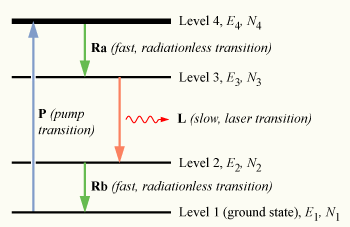
\includegraphics[scale=0.58]{bilder/Population-inversion-4level.png}
    \caption{Energieschema eines Vier-Zustandsystems \cite{wikipedia_population_inversion}.}
    \label{fig:4Niveau}
\end{figure}

Die Elektronen werden vom Grundzustand auf das Energieniveau 4 gepumpt. Von dort aus relaxiert das Elektron sehr schnell und ohne Emission von Strahlung in das Niveau 3. Der Übergang 
vom dritten Niveau zum zweiten Niveau findet über stimulierte Emission statt. Final relaxiert das Elektron vom zweiten Niveau in den Grundzustand zurück. Dort beginnt der Pump-Prozess
erneut. Durch konstantes pumpen bildet sich eine Besetzungsinversion. 

\section{Funktionsweise eines Halbleiterdiodenchips}
\label{sec:func_chip}

Eine Halbleiterdiode ist im Grunde nichts anderes als ein p-n Übergang. Ein p-n Übergang ist ein Kontakt bestehend aus einem p-dotierten und einem n-dotierten Halbleiter. N-Dotierung 
findet statt wenn ein Fremdatom in das Halbleitermaterial implantiert wird, welches mehr Valenzelektronen hat als das Halbleitermaterial. Das Fremdatom stellt in diesem Fall also ein
weiteres Elektron. P-Dotierung beschreibt dann genau das Gegenteil, also die Einbringung eines Fremdatoms mit weniger Valenzelektronen. Dieses Fremdatom bindet daher ein Elektronen.
Im Bandschema erzeugt Dotierung neue Zwischenniveaus. An der Kontaktfläche eines p-n Übergangs rekombinieren die Elektronen und Löcher. Es bildet sich eine Verarmungszone. In dieser 
Verarmungszone können sich keine freien Ladungsträger aufhalten und der Übergang wirkt isolierend. Legt man nun einen Strom an die Diode an, sodass der Pluspol an der p-Dotierung
anliegt, wirkt die anliegende Spannung dem intrinschen Potential entgegen. Die Elektronen und Löcher rekombinieren und emittieren ein Photon, welches ungefähr der Bandlücke entspricht. 
Das Valenz- und Leitungsband, sowie die Zwischenniveaus bilden ein Vier-Zustandsystem, weshalb eine Besetzngsinversion vorliegt. 

\section{Funktionsweise Diodenlaser}
\label{sec:func_dio}

Im innersten befindet sich ein in Abschnitt \ref{sec:func_chip} beschriebener Halbleiterdiodenchips. Durch anlegen eines Stroms wird kohärentes Licht emittiert. Die Forder- und 
Rückseite des Chips fungieren als Spiegel und bilden daher einen Resonator. Die Wellenlänge des emittierten Lichtes hängt von der Temperatur und dem Strom in der Diode ab. Der
Aufbau einer solchen Diode ist in Abbildung \ref{fig:LDChip} dargestellt. Das emittierte Licht ist sehr divergent, weshalb es durch eine Linse gebündelt werden muss. 

\begin{figure}
    \centering
    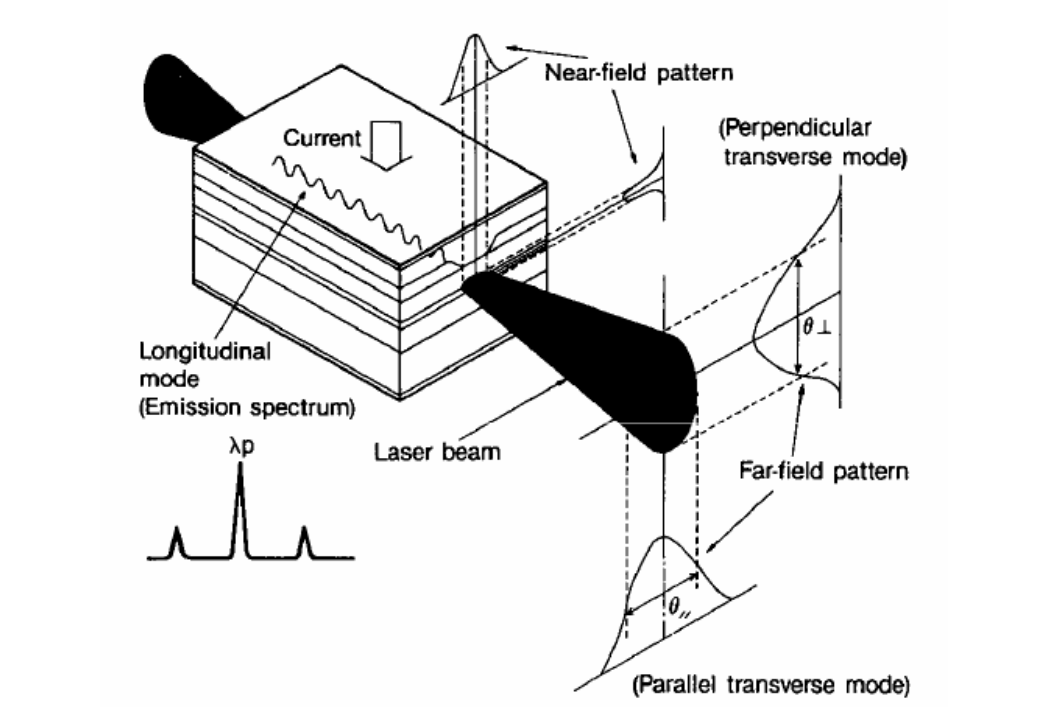
\includegraphics[scale=0.4]{bilder/LDChip.png}
    \caption{Schematische Abbildung eines Laser-Diodenchips. Es sind einzelne Schichten der Diode und eine stehende Welle erkennbar \cite{diode_laser_spectroscopy}.}
    \label{fig:LDChip}
\end{figure}

In einem Resonator der Länge $L$ mit dem Brechungsindex $n$ können Wellen der Wellenlängen $\lambda = \sfrac{2L}{k}  \;,k \in \mathbb{N}$ austreten. Diese weisen eine Frequenzbreite 
von 
\begin{equation}
    \label{eqn:delta_nu}
    \symup{\Delta} \nu = \frac{c}{2Ln}
\end{equation}
auf. Typische Frequenzbreiten eines einfachen Diodenlasers liegen im Bereich $\symup{\Delta} \nu \approx \qty{50}{\mega\hertz}$. Da dies für atomare Übergänge zu groß ist wird 
die Littrow-Konfiguration verwendet um diese Problem zu lösen. 

Die Littrow-Konfiguration ist in Abbildung \ref{fig:littrow} dargestellt.
\begin{figure}
    \centering
    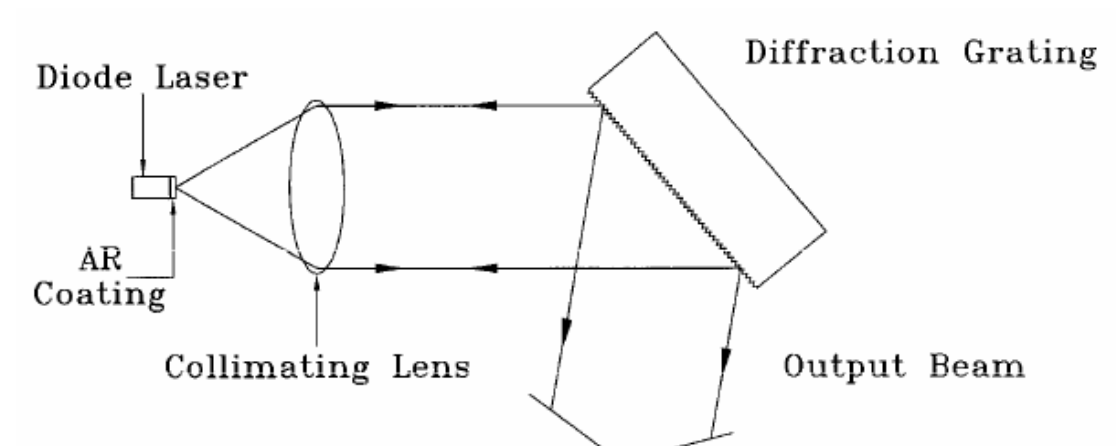
\includegraphics[scale=0.4]{bilder/aufbau_laser.png}
    \caption{Littrow-Konfiguration des Diodenlasers. \cite{diode_laser_spectroscopy}}
    \label{fig:littrow}
\end{figure}
Der Laserstrahl trifft auf das Gitter und wird dort zu $\qty{15}{\percent}$ in erster Beugungsordnung zurück in den Laser geworfen. Das Gitter und die hintere Wand des Diodenchips 
bilden daher einen äußeren Resonator größerer Länge. Daher sinkt die Frequenzbreite nach Gleichung \ref{eqn:delta_nu} auf einen kleineren Wert ab. Der restliche Anteil der Beugung am 
Gitter wird gemäß der Bragg-Bedingung 
\begin{equation}
    \label{eqn:Bragg}
    \lambda = 2d \sin\theta
\end{equation}
gebeugt, wobei $d$ der Gitterabstand und $\theta$ der Beugungswinkel ist. Da jede Wellenlänge anders gebeugt wird, kann anhand des Drehwinkels des Gitters die Wellenlänge verändert 
werden. 

\section{Frequenzvariation des Diodenlasers}
\label{sec:freq}

Im Diodenchip findet die Verstärkung in einem großen Bereich um eine zentrale Wellenlänge $\lambda_0$ statt. Dies tritt aufgrund der Banddispersion auf. Das Maximum ist dabei 
abhängig von der Temperatur und dem Diodenstrom. Bei Änderung der Temperatur kann sich allerdings auch der Brechungsindex ändern, weshalb sich die Mode ändern kann. Allerdings haben 
auch die anderen Bauteile einen Einfluss auf die verstärkte Wellenlänge. Der Zusammenhang der Bauteile wird in Abbildung \ref{fig:net_gain} dargestellt.

\begin{figure}
    \centering
    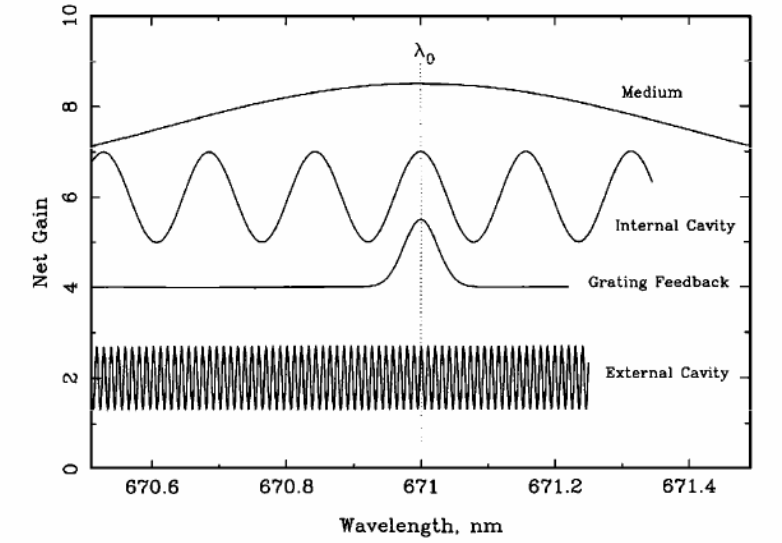
\includegraphics[scale=0.50]{bilder/net_gain.png}
    \caption{Verstärkungsfaktor der Komponenten in Abhängigkeit zur Wellenlänge. \cite{diode_laser_spectroscopy}.}
    \label{fig:net_gain}
\end{figure}

Die Temperaturabhänigkeit der Wellenlänge wird in Abbildung \ref{fig:temperatur} beschrieben.

\begin{figure}
    \centering
    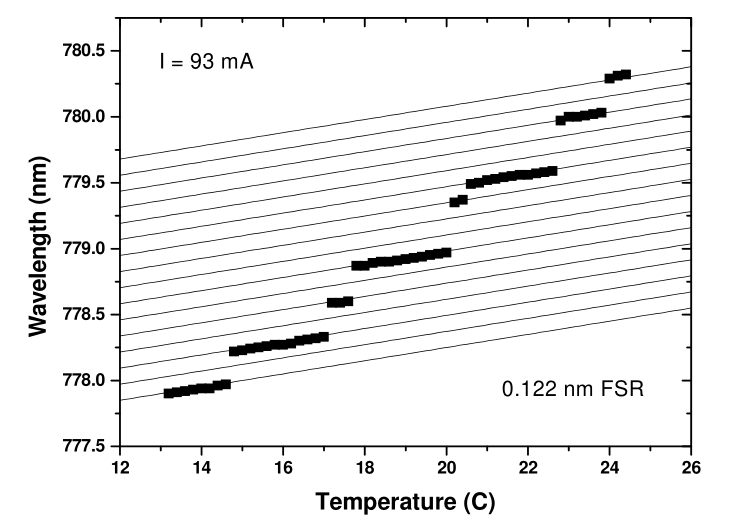
\includegraphics[scale=0.55]{bilder/temperatur.png}
    \caption{Temperaturabhänigkeit der verstärkten Wellenlänge einer Sanyo DL-7140-200S Diode \cite{diode_laser_spectroscopy}.}
    \label{fig:temperatur}
\end{figure}

Durch Abstimmen des inneren und des äußeren Resonators kann ein maximaler Gain gefunden werden. Dieses verhalten ist in Abbildung \ref{fig:moden} dargestellt.

\begin{figure}
    \centering
    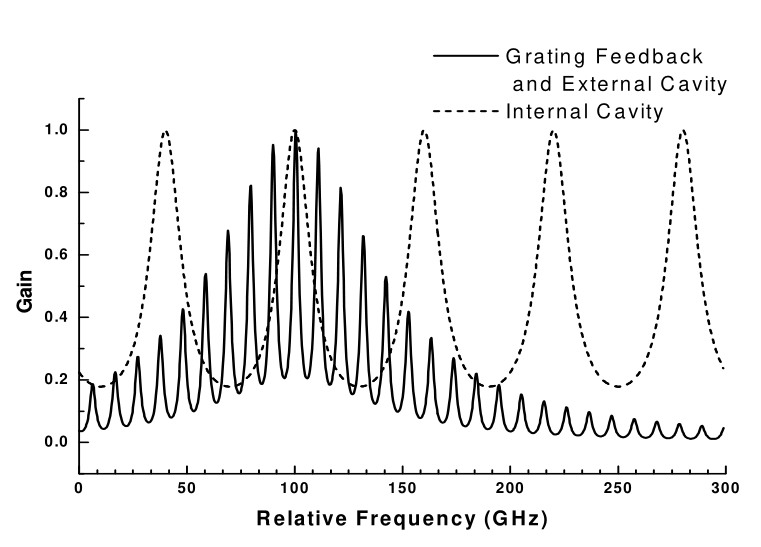
\includegraphics[scale=0.55]{bilder/moden.png}
    \caption{Abstimmung der Moden des inneren Resonators mit dem Spektrum des äußeren Resonators und des Gitters \cite{diode_laser_spectroscopy}.}
    \label{fig:moden}
\end{figure}

\section{Rubidium}
\label{sec:rub}

Rubidium ist ein Alkalimetall. Als solches eignet es sich besonders gut die Niveauaufspaltung durch Fein- und Hyperfeinstruktur zu beobachten, da eine qualitative Beschreibung nur 
für 1 Valenzelektronenatome existiert. Die Energieniveaus von Rubidium ist links in Abbildung \ref{spektrum_rubidium} zu entnehmen. Durch Photonen, welche genau der Energiedifferenz der Niveaus 
entsprechen können die Photonen absorbiert werden und das Elektron anregen. Relaxieren diese Elektronen wieder senden sie ein Photon der selben Wellenlänge aus. Auch wenn diese 
Photonen in alle Raumrichtungen emittiert werden, können sie detektiert werden.

Wird der Laserstrahl nun auf ein Rubidiumgas geschickt und das transmitierte Spektrum aufgenommen, so ist die Intensität genau der Anregungswellenlängen sehr gering. Das erwartete 
Absorptionsspektrum von Rubidium ist rechts in Abbildung \ref{fig:spektrum_rubidium} dargestellt.

\begin{figure}
    \centering
    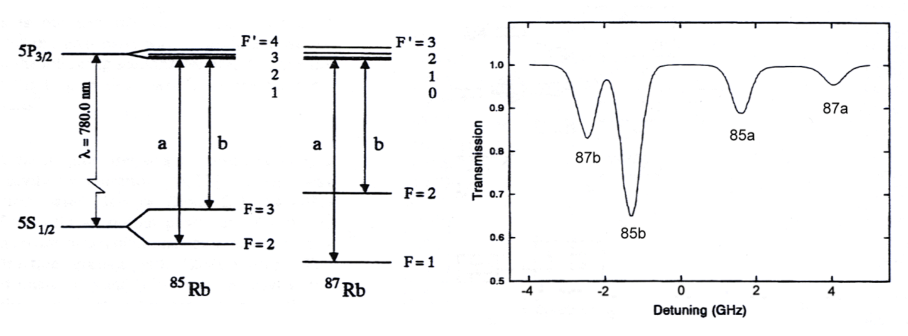
\includegraphics[scale=0.55]{bilder/spektrum_rubidium.png}
    \caption{Energieniveaus von Rubidium, sowie das daraus resultierende Absorptionsspektrum \cite{diode_laser_spectroscopy}.}
    \label{fig:spektrum_rubidium}
\end{figure}

\input{content/03_durchführung.tex}
\chapter{Analysis}
\label{cha:analysis}

After the setup was adjusted the first measurement is taken. The data shown in plot \ref{fig:no_purge}. 



The maxium of the plot lies at around $\qty{153645}{a.u.}$ of electric field amplitude.

Here will come some words as an introduction. maybe about the amplitude of the null measurement so that the basis of the measurement is clear.

\section{Air Humidity in the Laboratory}
\label{sec:water_abso}
To extract frequency information a fast fourier transformation (FFT) of the data is performed. The frequency domain is represented in figure \ref{fig:freq_no_purge}.


\chapter{Diskussion}
\label{cha:Diskussion}
Im ersten Teil des Versuches wurde der Kontrast des Interferometers bestimmt. Der Kontrast hängt von der Justierung des Interferometers ab und sollte möglichst nach an $K = 1$ sein.
Der maximale Kontrast der durchgeführten Justierung liegt bei $K_\mathrm{max} = 0.9608$. Dieser Wert ist sehr nach an einer idealen Justierung, daher kann von einem qualitativen Aufbau
ausgegangen werden von welchen auch qualitative Messwerte erwartet werden können. Dies zeigt sich im nächsten Teil des Versuches. 

Nun wurde der Brechungsindex von Glas bestimmt. Dabei
ergibt sich bei einem Messwert von $\num{1.5228 \pm 0.0124}$ eine relative Abweichung zum Theoriewert $n_{Theo} = \num{1.52}$\cite{phy-chem-eigenschaften} von $\Delta n_\mathrm{Glas} = \qty{0.2}{\percent}$. Dies ist eine sehr kleine Abweichung, 
welche allerdings nur gilt, wenn das verwendete Glas normales Fensterglas ist. Leider liegt keine Information darüber vor, weshalb diese Annahme getroffen wurde.

Im letzten Teil des Versuches wurde der Brechungsindex von Luft bestimmt. Hier ergibt sich eine relative Abweichung zum Literaturwert $n_{\mathrm{L,Theo}} = 1.000292$ \cite{Ingenieurwissen} von $\Delta n_\mathrm{Luft} = \qty{5.41}{\percent}$.
Diese Abweichung ist ebenfalls sehr gering. Die kleinen Abweichungen können die gute Justierung bestätigen. 

Nichts desto trotz sorgen kleine Abweichung in der äußeren Bedingungen oder kleine Positionsänderungen der Spiegel und Würfel für relativ große Änderungen im Interferenzeffekt. Daher 
bietet sich hier eine mögliche Quelle für Unsicherheiten. Außerdem können, obwohl der Aufbau durch eine Purgebox vor Luftschwankungen geschützt wurde, Luftschwankungen einen Einfluss haben.
Ebenfalls kann ein systematischer Fehler in Form von nicht perfekter Einstellung der Differenzspannungsmethode auftreten wodurch Maxima nicht vollständig aufgenommen werden. Dies liegt 
daran, dass auch hintergrundrauschen für mögliche Nulldurchgänge sorgen kann.

Zusammengefasst wurde das Experiment durch alle möglichen Schutzmaßnahmen vor äußeren Einflüssen bewahrt und das Experiment wurde erfolgreich durchgeführt und liefert zufriedenstellende Ergebnisse. 

%\mainmatter
%\newpage


%\backmatter
\printbibliography

\chapter*{Anhang}
\label{cha:Messdaten}

%Hier können die aufgenommenen Messdaten angehangen werden
\addcontentsline{toc}{chapter}{Anhang}

\begin{table}
    \centering
    \caption{Emissionswahrscheinlichkeiten $W$ der FEP für Europium-152 sotiert nach $W$. \cite{Gammaspektrum_Eu152}}
    \label{tab:eu152_FEP}
    \begin{tabular}{c c}
      \toprule
      $E \mathbin{/} \unit{\kilo\electronvolt}$ & $W \mathbin{/} \% $ \\
      \midrule
      $\qty{121.78}{} $ & $\qty{28.58}{}$ \\
      $\qty{344.28}{}$ & $\qty{26.5}{}$ \\
      $\qty{1408.01}{}$ & $\qty{21.01}{}$  \\
      $\qty{964.08}{}$ & $\qty{14.61}{}$  \\
      $\qty{1112.07}{}$ & $\qty{13.64}{}$\\
      $\qty{778.90}{}$ & $\qty{12.94}{}$  \\
      $\qty{1085.87}{}$ & $\qty{10.21}{}$ \\
      $\qty{244.70}{}$ & $\qty{7.58}{}$  \\
      $\qty{867.38}{}$ & $\qty{4.25}{}$  \\
      $\qty{443.965}{}$ & $\qty{2.82}{}$ \\
      $\qty{411.12}{}$ & $\qty{2.23}{}$  \\
      $\qty{1089.74}{}$ & $\qty{1.73}{}$ \\
      $\qty{1299.14}{}$ & $\qty{1.62}{}$ \\
      $\qty{1212.95}{}$ & $\qty{1.42}{}$ \\

      \bottomrule
    \end{tabular}
\end{table}

\end{document}
